\section{Castalia Application Layer}\label{castaliaapplayer}

We create a application to the Castalia Application Layer. This application is agent-initiated, that is, the agent takes the initiative to send readings to the manager. The agents is the first and the only to send the association request to start sending measurements and the association release when there is no more measurements to be sent.

The current code has five agents implemented, a pulse oximeter, glucose meter, thermometer, blood pressure, and a basic ECG. The pulse oximeter transmit data like the pulse rate in beats per second and the Percentage of arterial haemoglobin oxygen saturation (SpO$_2$). The glucose meter convey the glucose level, that is, the concentration of blood sugar in the blood in milligrams per deciliter (mg\//dL) and the thermometer the temperature is in Celsius degree (\textdegree C). The blood pressure sends a data compound of systolic, diastolic and the mean arterial pressure in millimeters of mercury (mmHg). The basic ECG sends eighty samples values in each packet, each value is a millivolt (mV) sample. In the basic ECG, the seconds spacing between the samples is sent in the configuration phase as well as the lower and upper absolute value and the lower and upper scaled value. All this values are randomly produced except for basic ECG that transmit real values obtained from the data base \cite{b2}. 

The 11073 standard define confirmed and unconfirmed events. The confirmed events are message that expected an acknowledgment and the unconfirmed events doesn't expect a confirmation. Messages like \textit{Association request} and \textit{Association release} always has acknowledgments but measurements messages can be confirmed or unconfirmed. %The implemented parameter to set the desired mode is \textit{SN.node\[node number\].Application.confirmed\_event} which require a Boolean value.

\subsection{Unconfirmed measurement event}\label{sec:UnconfirmedMeasurementEvent}

Fig.\ref{fig:unconfirmedMode} shows a sequence diagram of the messaging procedure corresponding to a ordinary operation of an agent with standard configuration. The agent intends to associate with the manager for the first time and sends a \textit{Association request}. When the manager receives the \textit{Association request} it checks if there was some association made before. If not it sends an \textit{Get attributes} message along with the \textit{Association response}. So the agent sends its configuration and start to convey the measurements to the manager. When there is no more readings to transmit the agent sends a \textit{Association release} and the manager responds with an \textit{Association release response}.

\begin{figure}[htbp]
\centerline{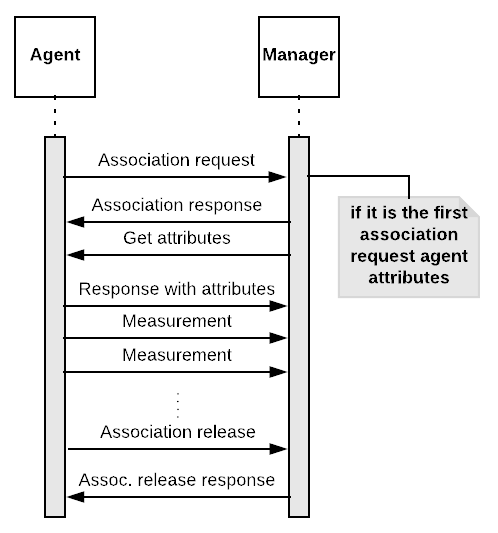
\includegraphics[scale=0.35]{figures/unconfirmed.png}}
\caption{Sequence diagram of unconfirmed operation mode of an 11073 PHD application.}
\label{fig:unconfirmedMode}
\end{figure}

\subsection{Confirmed measurement event}

\begin{figure}[htbp]
\centerline{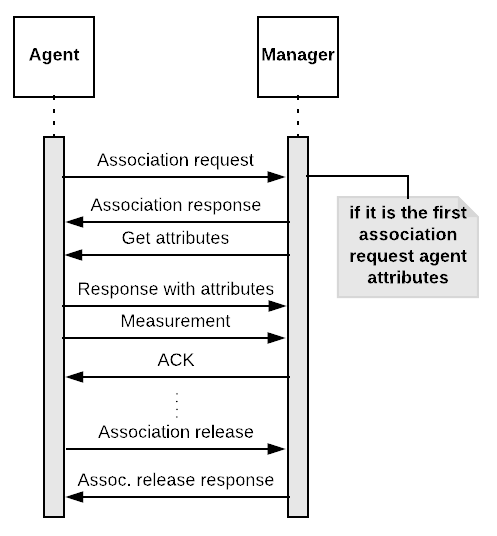
\includegraphics[scale=0.35]{figures/confirmed.png}}
\caption{Sequence diagram of confirmed operation mode of an 11073 PHD application.}
\label{fig:confirmedMode}
\end{figure}

Now the Fig.\ref{fig:confirmedMode} depicts a sequence diagram of the messaging procedure corresponding to an operation of an agent with standard configuration and with confirmed measurements events. The initial procedure is the same as explained at Section \ref{sec:UnconfirmedMeasurementEvent}. The difference is that the manager sends an acknowledgment for every measurement received. After sending a measurement data the agent shall wait three seconds. If an answer is not received in this period the agent shall send an \textit{Association abort} to the manager and transition back to the unassociated state. If the agent still has readings to send a new association must be done. This and others errors conditions is explained in \cite{b1}.

\subsection{Proposed modification in confirmed measurement event}

The 11073 standard assumes that there will be a transport layer on real devices. In the Castalia simulator as in other wireless sensor networks we do not have a transport layer, so a stop-and-wait system was implemented at the application layer for retransmission of packets that did not receive a confirmation ACK. This modification avoid many associations right after a non-received ACK.

%To avoid many associations right after a non-received ACK we implemented a stop-and-wait retransmission system in the application layer. 
This save the unnecessary exchange of several control packets. Rather than making a new association we just retransmit the packet $n$ times or until an ACK from manger is received.
%The user can define whether to retransmit and how many retransmission attempts wish.
If an ACK from the manager is lost, the agent will try to retransmit the packet $n$ times as defined by the user. When the manager finally receives the packet, it will retransmit immediately the lost ACK to the agent.

Will be shown in Results Section how this system can save many control packets exchanged when a ACK is not received. Note that this is an independent modification, not present in the 11073 standard. 
%The parameters implemented for retransmission are \textit{SN.node[nodeNumber].Application.retransmissionPacket} which require a boolean value and \textit{SN.node[nodeNumber].Application.maxNumOfRetransmition} that accepts an integer number.